\documentclass[11pt]{article}
\usepackage{amsmath}
\usepackage{hyperref}
\usepackage{listings}
\usepackage{xcolor}
\usepackage{pdfpages}
\usepackage{graphicx}
\usepackage{subcaption}
\usepackage{float}

\topmargin=-0.45in
\evensidemargin=0in
\oddsidemargin=0in
\textwidth=6.5in
\textheight=9.0in
\headsep=0.25in

\renewcommand{\thesubsection}{\alph{subsection})}
\renewcommand{\thesubsubsection}{\roman{subsubsection}.}

% Title and Author Customization
\title{
    \vspace{3em}
    \textbf{Deep Learning: ECE-7123}\\
    Homework 3
    \vspace{1em}
}

\author{
    Saad Zubairi \\ 
    shz2020 \\
    \vspace{1em}
}

\vspace{1em}
\date{May 2, 2025}

\begin{document}
\maketitle	
\pagebreak

\tableofcontents

\pagebreak

\section{Problem 1: Minimax optimization}

Given the function:

\[
\min_x \max_y f(x, y) = 4x^2 - 4y^2.
\]

Which can be plotted as:

\begin{center}
    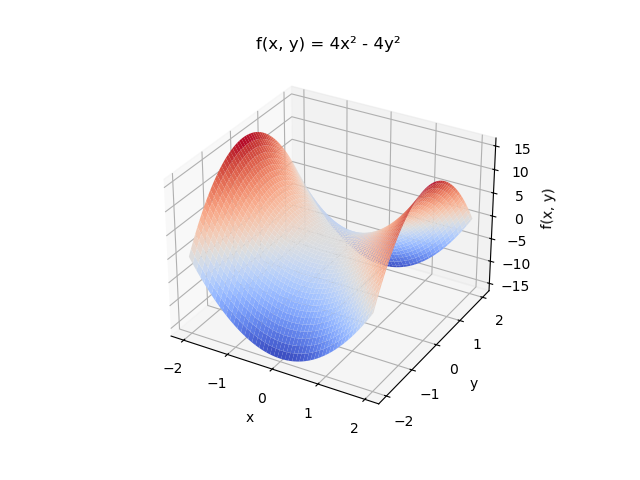
\includegraphics[scale=0.5]{Q1/plot.png}
\end{center}

\subsection{Saddle point}

To find the saddle point, we can take the partial derivatives with respect to \(x\) and \(y\):

\[
\nabla f(x, y) = \left( \frac{\partial f}{\partial x}, \frac{\partial f}{\partial y} \right) = (8x, -8y)
\]
Setting \(\nabla f(x, y) = 0\), we solve:
\[
8x = 0 \quad \text{and} \quad -8y = 0
\]

This gives the saddle point at \((x, y) = (0, 0)\).

\subsection{Gradient descent/ascent update rules}

To derive the update rules for gradient descent in \(x\) and gradient ascent in \(y\), we start with the function \(f(x, y) = 4x^2 - 4y^2\). The gradient of \(f(x, y)\) is given by:

\[
\nabla f(x, y) = \left( \frac{\partial f}{\partial x}, \frac{\partial f}{\partial y} \right) = (8x, -8y).
\]

For gradient descent in \(x\), we update \(x\) by moving in the direction opposite to the gradient:

\[
x_{t+1} = x_t - \eta \frac{\partial f}{\partial x}.
\]

Substituting \(\frac{\partial f}{\partial x} = 8x_t\), we get:

\[
x_{t+1} = x_t - \eta (8x_t) = x_t (1 - 8\eta).
\]

For gradient ascent in \(y\), we update \(y\) by moving in the direction of the gradient:

\[
y_{t+1} = y_t + \eta \frac{\partial f}{\partial y}.
\]

Substituting \(\frac{\partial f}{\partial y} = -8y_t\), we get:

\[
y_{t+1} = y_t + \eta (-8y_t) = y_t (1 + 8\eta).
\]

Thus, the update rules are:

\[
x_{t+1} = (1 - 8\eta)x_t, \quad y_{t+1} = (1 + 8\eta)y_t.
\]

\subsection{Convergence of the update rules}

To ensure convergence, we analyze the update rules:

\[
x_{t+1} = (1 - 8\eta)x_t, \quad y_{t+1} = (1 + 8\eta)y_t.
\]

For convergence of \(x_t\) in gradient descent, the factor \((1 - 8\eta)\) must satisfy:

\[
|1 - 8\eta| < 1.
\]

Solving this inequality:

\[
-1 < 1 - 8\eta < 1.
\]

Subtracting 1 from all sides:

\[
-2 < -8\eta < 0.
\]

Dividing through by \(-8\) (reversing the inequality):

\[
0 < \eta < \frac{1}{4}.
\]

For \(y_t\) in gradient ascent, the factor \((1 + 8\eta)\) must satisfy:

\[
|1 + 8\eta| < 1.
\]

Solving this inequality:

\[
-1 < 1 + 8\eta < 1.
\]

Subtracting 1 from all sides:

\[
-2 < 8\eta < 0.
\]

Dividing through by \(8\):

\[
-\frac{1}{4} < \eta < 0.
\]

Since \(\eta\) must be positive for gradient descent and ascent to make sense, we combine the results:

\[
0 < \eta < \frac{1}{4}.
\]

Thus, the range of allowable step sizes is:

\[
\boxed{0 < \eta < \frac{1}{4}}
\]

\subsection{Regular gradient descent on both variables}

To analyze regular gradient descent on both variables \(x\) and \(y\), we update both using the gradient of \(f(x, y)\). The gradient is:

\[
\nabla f(x, y) = (8x, -8y).
\]

The update rules for gradient descent on \(x\) and \(y\) are:

\[
x_{t+1} = x_t - \eta \frac{\partial f}{\partial x}, \quad y_{t+1} = y_t - \eta \frac{\partial f}{\partial y}.
\]

Substituting the partial derivatives:

\[
x_{t+1} = x_t - \eta (8x_t) = x_t (1 - 8\eta),
\]
\[
y_{t+1} = y_t - \eta (-8y_t) = y_t (1 + 8\eta).
\]

Thus, the update rules are:

\[
x_{t+1} = (1 - 8\eta)x_t, \quad y_{t+1} = (1 + 8\eta)y_t.
\]

Dynamics of the updates

\begin{itemize}
    \item For \(x_t\), the factor \((1 - 8\eta)\) determines the convergence. If \(0 < \eta < \frac{1}{4}\), then \(|1 - 8\eta| < 1\), ensuring that \(x_t\) decays to 0.
    \item For \(y_t\), the factor \((1 + 8\eta)\) determines the behavior. Since \((1 + 8\eta) > 1\) for \(\eta > 0\), \(y_t\) grows exponentially, leading to divergence.
\end{itemize}

% \subsubsection{Conclusion}

% Regular gradient descent on both variables does not converge to the saddle point unless \(y_0 = 0\) exactly and remains unperturbed. This is because \(y_t\) diverges due to the exponential growth caused by \((1 + 8\eta) > 1\).

\section{Vision-Language models}

\subsection*{Overview}
In this experiment, we evaluate three different combinations of image and text encoders for CLIP-style contrastive learning. The goal is to assess how different architectural choices affect the model’s ability to align images and captions.

\subsection*{Model Configurations}
\subsubsection*{Combination 1: ResNet-50 + DistilBERT}
\begin{itemize}
    \item Image Encoder: \texttt{resnet50} (output dim: 2048)
    \item Text Encoder: \texttt{distilbert-base-uncased} (output dim: 768)
    \item Projection Dim: 256
\end{itemize}

\subsubsection*{Combination 2: ResNet-18 + BERT}
\begin{itemize}
    \item Image Encoder: \texttt{resnet18} (output dim: 512)
    \item Text Encoder: \texttt{bert-base-uncased} (output dim: 768)
    \item Projection Dim: 256
\end{itemize}

\subsubsection*{Combination 3: ResNet-34 + RoBERTa}
\begin{itemize}
    \item Image Encoder: \texttt{resnet34} (output dim: 512)
    \item Text Encoder: \texttt{roberta-base} (output dim: 768)
    \item Projection Dim: 256
\end{itemize}

\subsection{Rationale}
The encoder combinations were selected semi-randomly to reflect varying model scales. The purpose is to observe whether larger encoders (e.g., ResNet-50, RoBERTa) yield visibly better alignment without tuning hyperparameters.

\subsection{Implementation Changes}

\subsubsection*{Config Changes}
All modifications are made in the \texttt{config} class.

\begin{verbatim}
    model_name = 'resnet50'
    image_embedding = 2048
    text_encoder_model = 'roberta-base'
    text_tokenizer = 'roberta-base'
    text_embedding = 768
    projection_dim = 512
\end{verbatim}

\subsubsection*{Encoder Changes}
In addition to updating the \texttt{config} class, the encoders were modified throughout the implementation to support RoBERTa. This included:

\begin{itemize}
    \item Updating the forward pass to handle RoBERTa's tokenization and embedding outputs.
    \item Adjusting the projection layers to match the output dimensions of RoBERTa (768) and the specified projection dimension (256).
    \item Updating the \texttt{get\_image\_embeddings} function to use \texttt{AutoTokenizer} for tokenization; compaitble with the updated \texttt{text\_tokenizer}.
\end{itemize}

\subsection{Inference Examples}

\subsubsection{Prompt: ``A cat sitting with a human''}
\vspace{0.5em}

\begin{figure}[H]
    \centering
    \begin{subfigure}[b]{0.3\textwidth}
        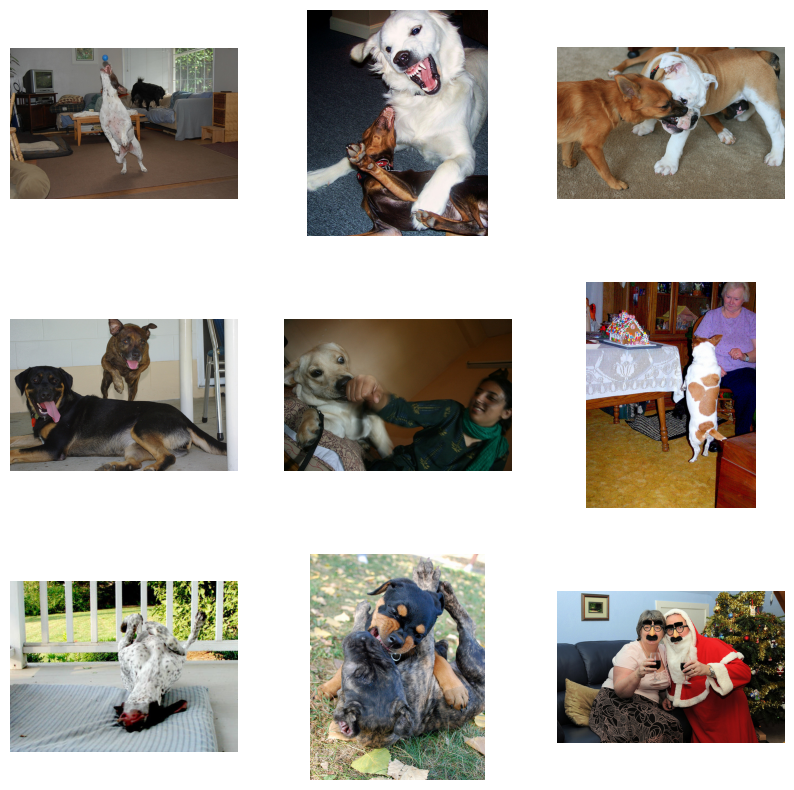
\includegraphics[width=\linewidth]{Q2/A cat sitting with a human/1.png}
        \caption{\tiny ResNet-50 + DistilBERT}
    \end{subfigure}
    \hfill
    \begin{subfigure}[b]{0.3\textwidth}
        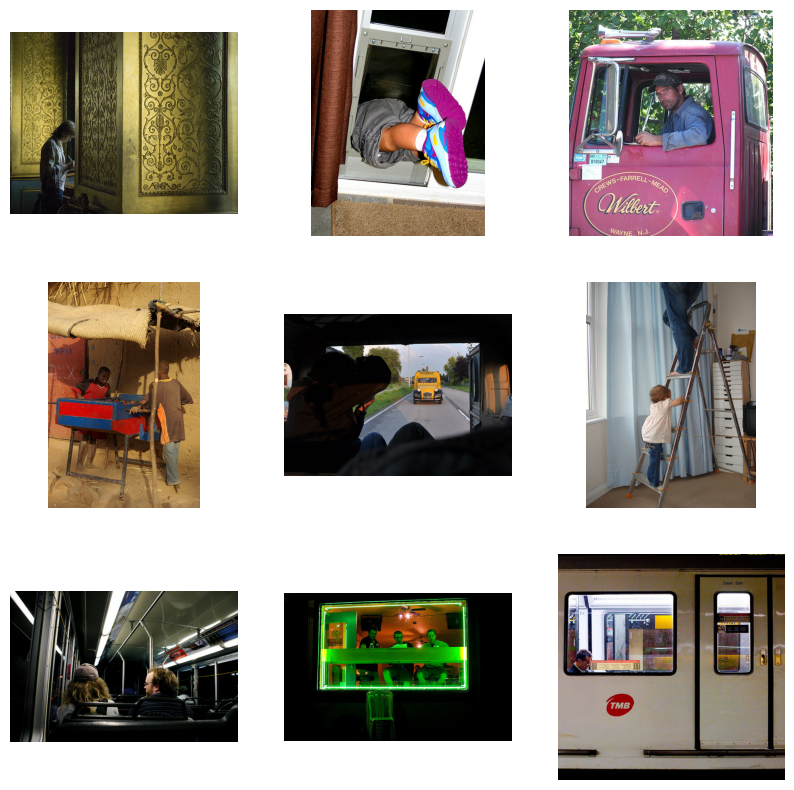
\includegraphics[width=\linewidth]{Q2/A cat sitting with a human/2.png}
        \caption{\tiny ResNet-18 + BERT}
    \end{subfigure}
    \hfill
    \begin{subfigure}[b]{0.3\textwidth}
        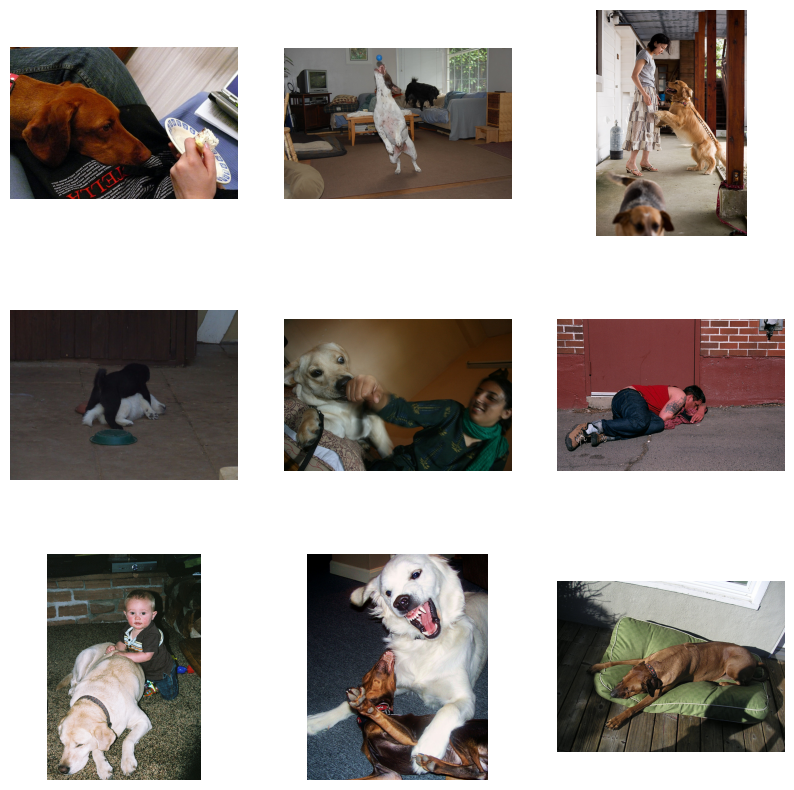
\includegraphics[width=\linewidth]{Q2/A cat sitting with a human/3.png}
        \caption{\tiny ResNet-34 + RoBERTa}
    \end{subfigure}
    
\end{figure}

\subsubsection{Prompt: ``A crowd gathered in a park''}
\vspace{0.5em}

\begin{figure}[H]
    \centering
    \begin{subfigure}[b]{0.3\textwidth}
        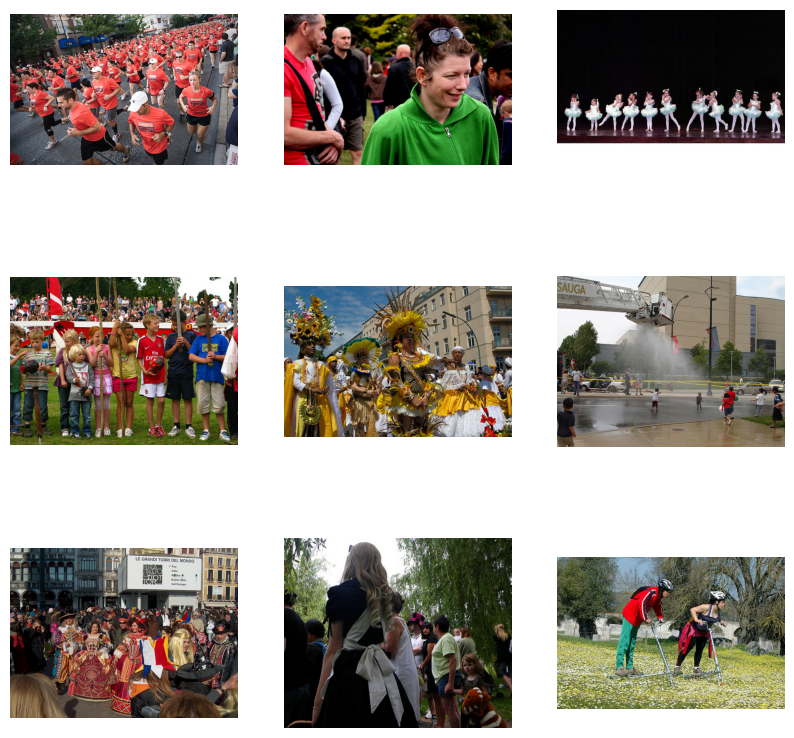
\includegraphics[width=\linewidth]{Q2/A crowd gathered in a park/1.png}
        \caption{\tiny ResNet-50 + DistilBERT}
    \end{subfigure}
    \hfill
    \begin{subfigure}[b]{0.3\textwidth}
        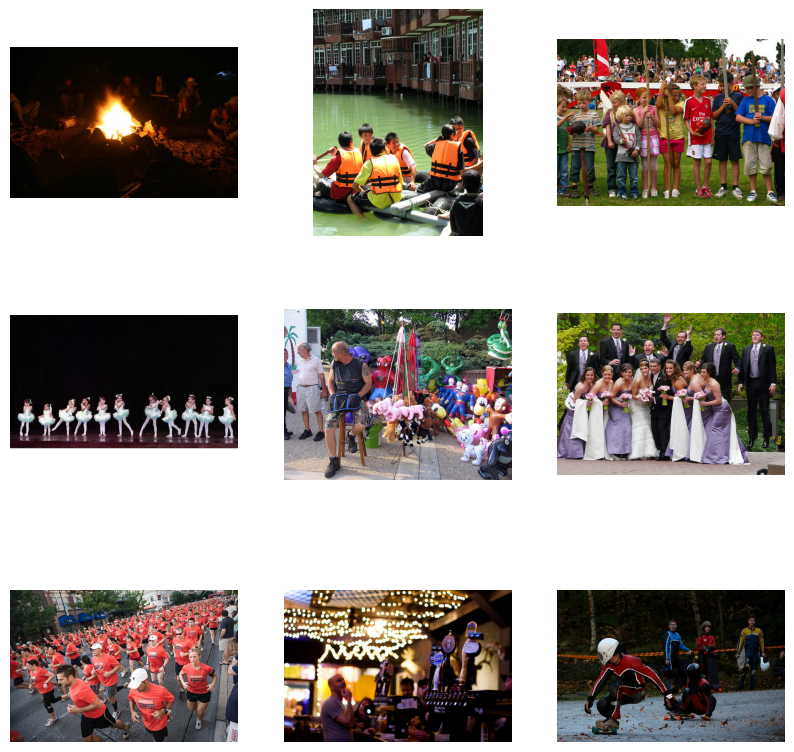
\includegraphics[width=\linewidth]{Q2/A crowd gathered in a park/2.png}
        \caption{\tiny ResNet-18 + BERT}
    \end{subfigure}
    \hfill
    \begin{subfigure}[b]{0.3\textwidth}
        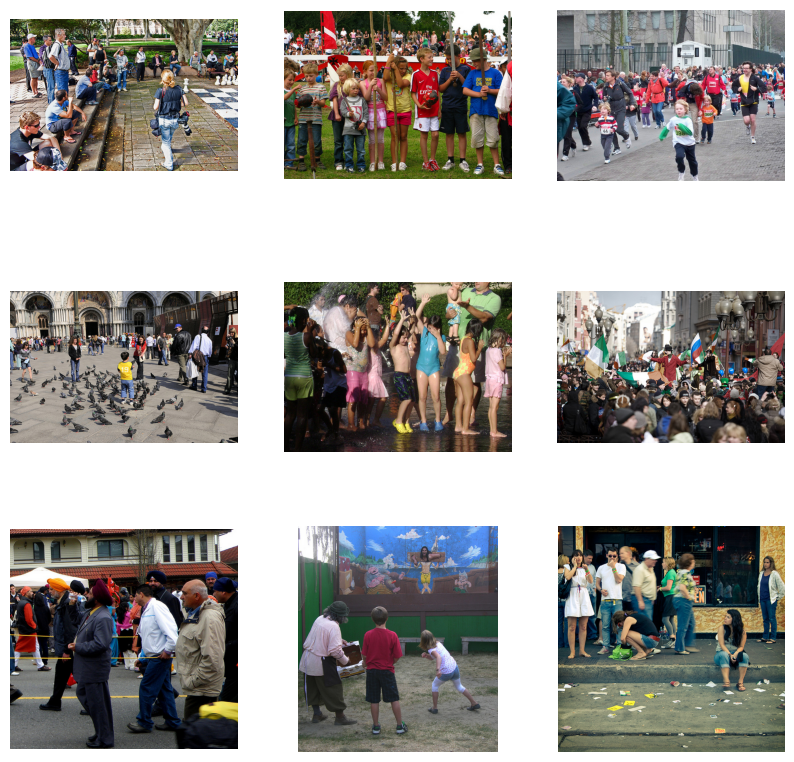
\includegraphics[width=\linewidth]{Q2/A crowd gathered in a park/3.png}
        \caption{\tiny ResNet-34 + RoBERTa}
    \end{subfigure}
    
\end{figure}

\subsubsection{Prompt: ``A dog sitting alone in a park''}
\vspace{0.5em}

\begin{figure}[H]
    \centering
    \begin{subfigure}[b]{0.3\textwidth}
        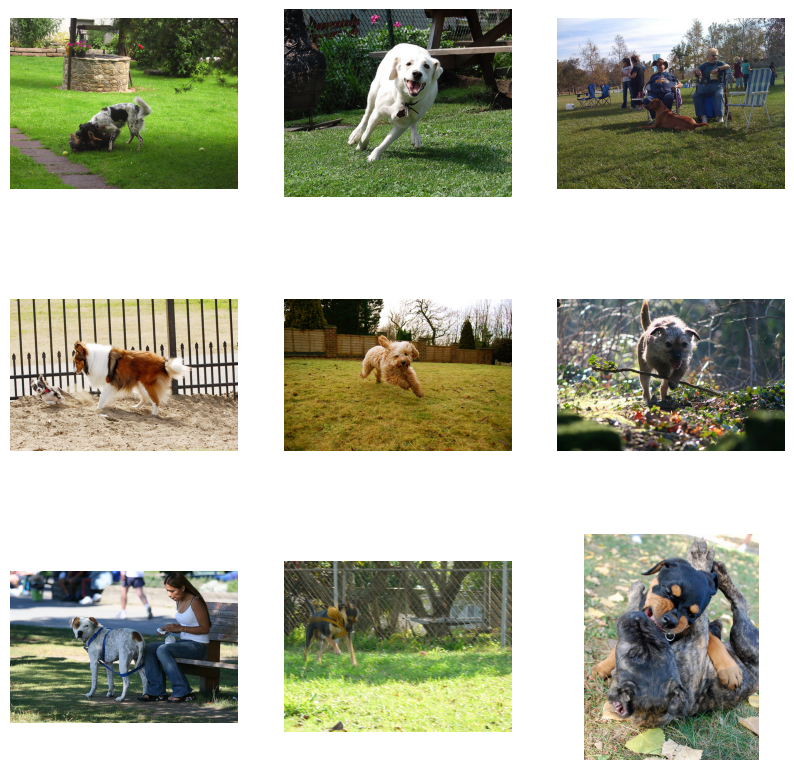
\includegraphics[width=\linewidth]{Q2/A dog sitting alone in a park/1.png}
        \caption{\tiny ResNet-50 + DistilBERT}
    \end{subfigure}
    \hfill
    \begin{subfigure}[b]{0.3\textwidth}
        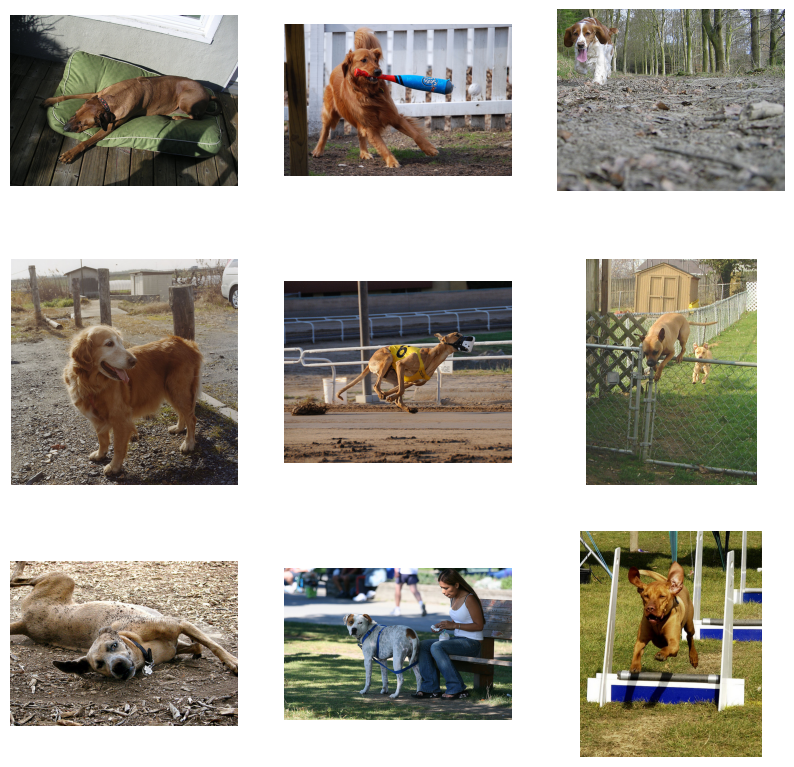
\includegraphics[width=\linewidth]{Q2/A dog sitting alone in a park/2.png}
        \caption{\tiny ResNet-18 + BERT}
    \end{subfigure}
    \hfill
    \begin{subfigure}[b]{0.3\textwidth}
        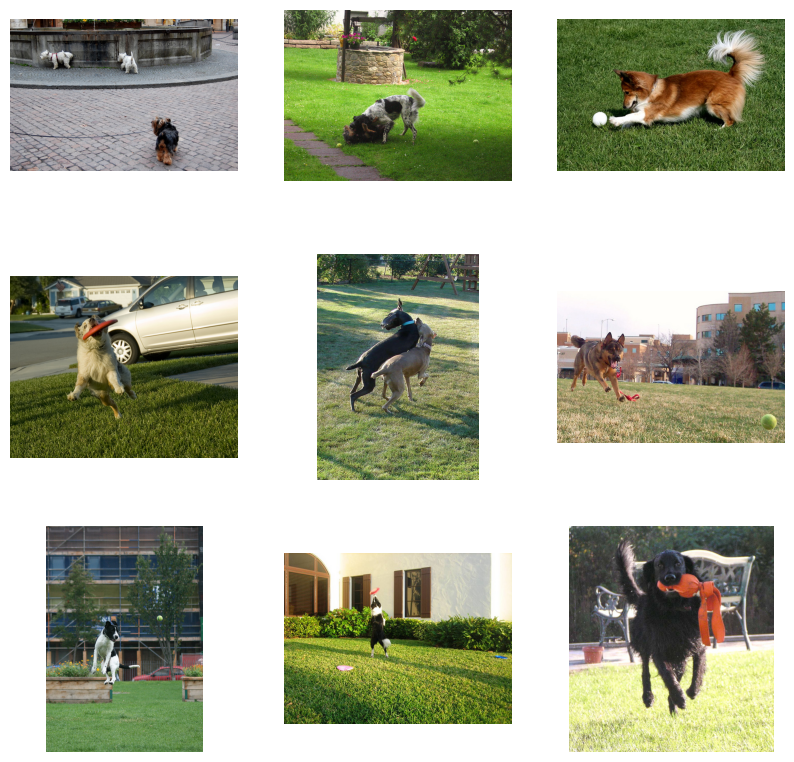
\includegraphics[width=\linewidth]{Q2/A dog sitting alone in a park/3.png}
        \caption{\tiny ResNet-34 + RoBERTa}
    \end{subfigure}
    
\end{figure}

\subsubsection{Prompt: ``A man skateboarding in the city''}
\vspace{0.5em}

\begin{figure}[H]
    \centering
    \begin{subfigure}[b]{0.3\textwidth}
        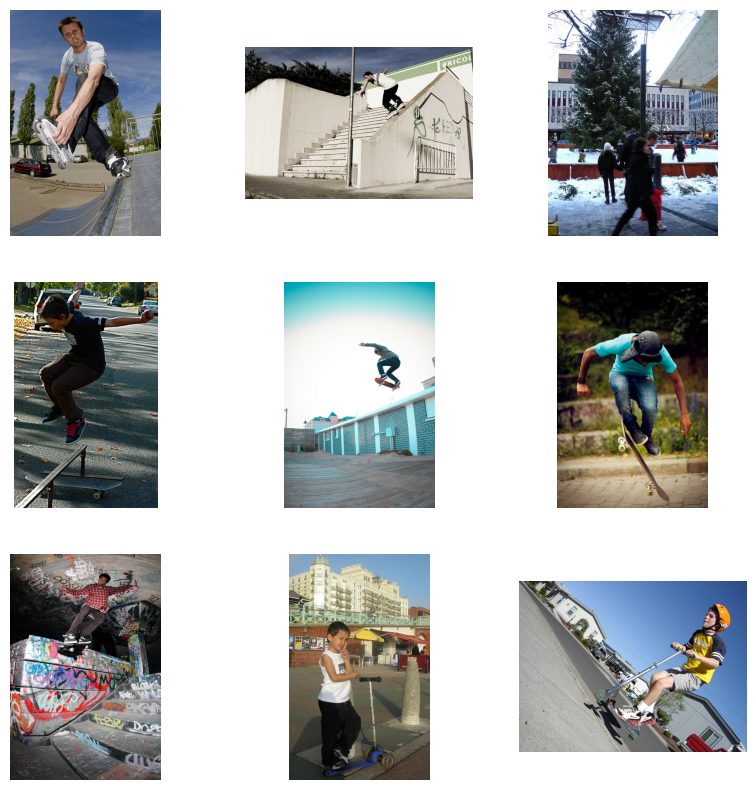
\includegraphics[width=\linewidth]{Q2/A man skateboarding in the city/1.png}
        \caption{\tiny ResNet-50 + DistilBERT}
    \end{subfigure}
    \hfill
    \begin{subfigure}[b]{0.3\textwidth}
        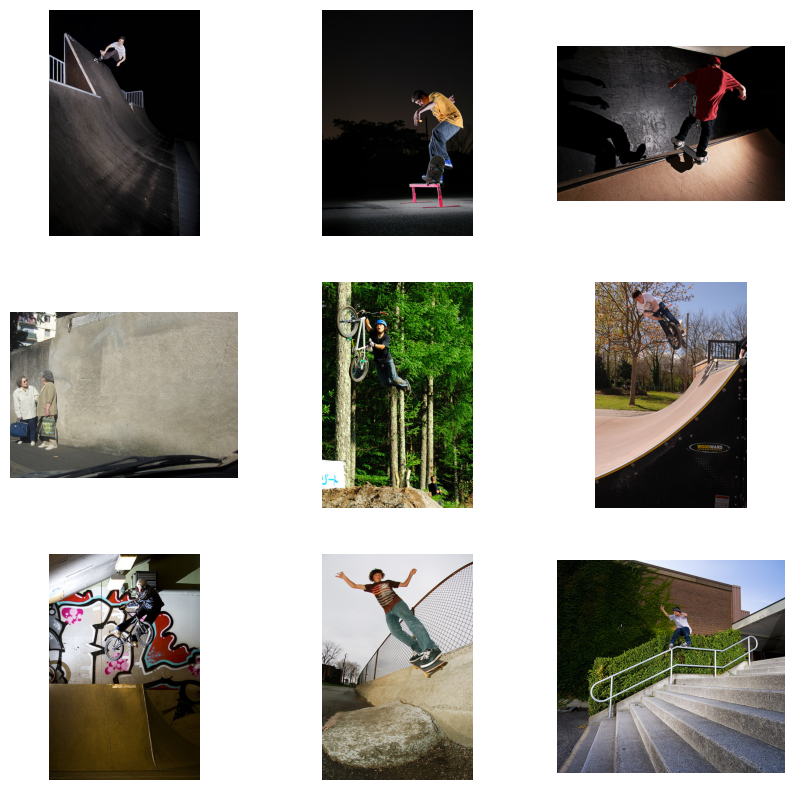
\includegraphics[width=\linewidth]{Q2/A man skateboarding in the city/2.png}
        \caption{\tiny ResNet-18 + BERT}
    \end{subfigure}
    \hfill
    \begin{subfigure}[b]{0.3\textwidth}
        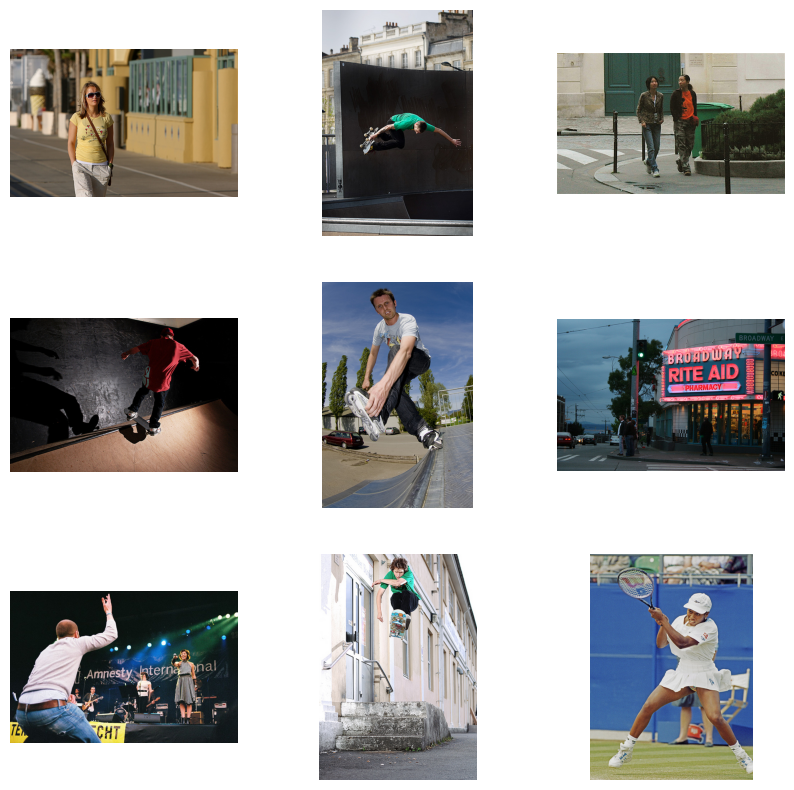
\includegraphics[width=\linewidth]{Q2/A man skateboarding in the city/3.png}
        \caption{\tiny ResNet-34 + RoBERTa}
    \end{subfigure}
    
\end{figure}

\subsubsection{Prompt: ``All kinds of food on a table''}
\vspace{0.5em}

\begin{figure}[H]
    \centering
    \begin{subfigure}[b]{0.3\textwidth}
        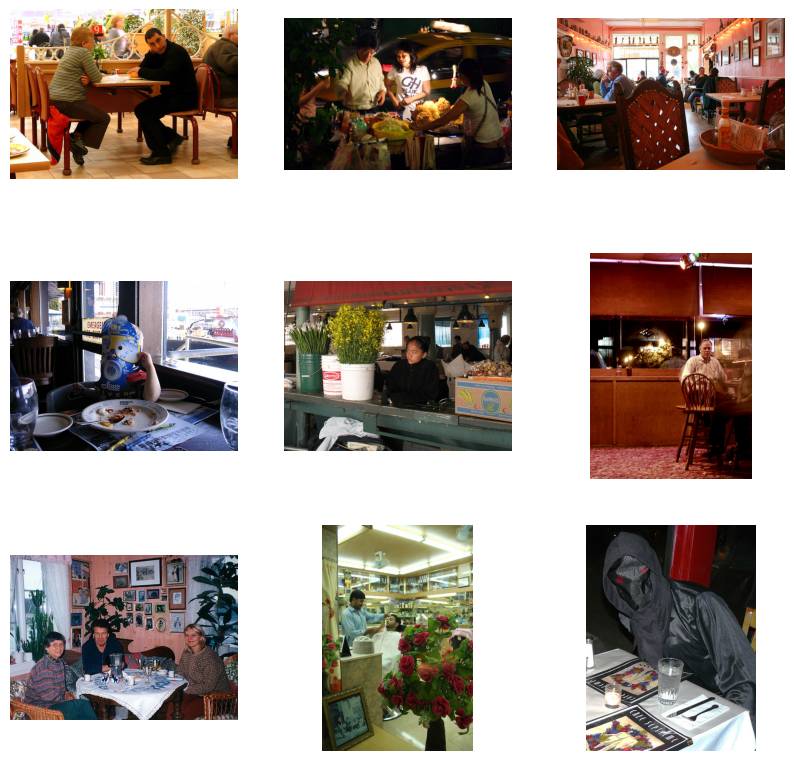
\includegraphics[width=\linewidth]{Q2/All kinds of food on a table/1.png}
        \caption{\tiny ResNet-50 + DistilBERT}
    \end{subfigure}
    \hfill
    \begin{subfigure}[b]{0.3\textwidth}
        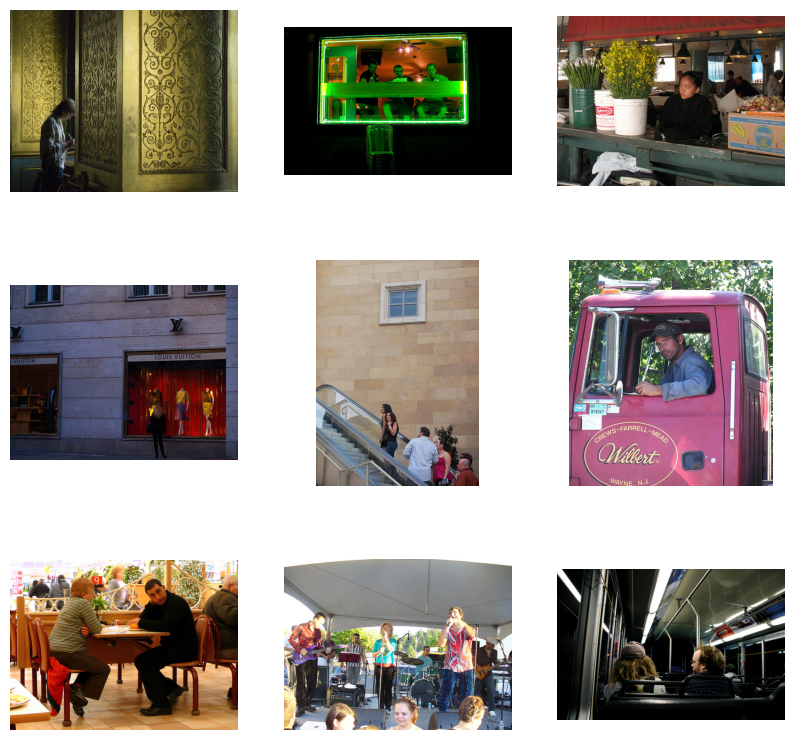
\includegraphics[width=\linewidth]{Q2/All kinds of food on a table/2.png}
        \caption{\tiny ResNet-18 + BERT}
    \end{subfigure}
    \hfill
    \begin{subfigure}[b]{0.3\textwidth}
        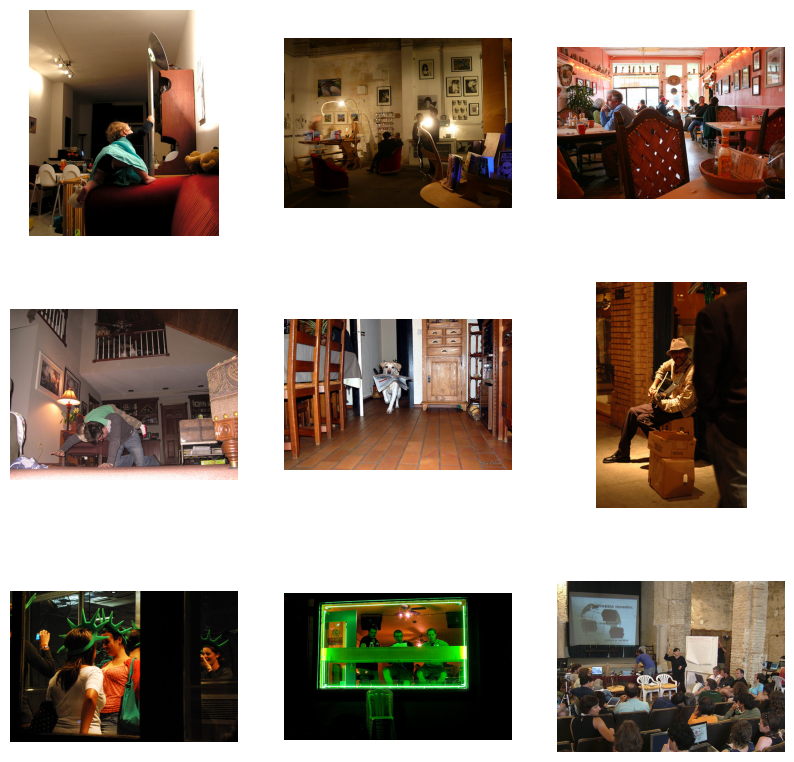
\includegraphics[width=\linewidth]{Q2/All kinds of food on a table/3.png}
        \caption{\tiny ResNet-34 + RoBERTa}
    \end{subfigure}
    
\end{figure}

\subsection{Evaluation}

\subsubsection{Prompt: ``A cat sitting with a human''}
This prompt revealed major limitations across all models.

\begin{itemize}
    \item \textbf{Model A:} Returned dog images—incorrect, but at least animal-adjacent.
    \item \textbf{Model B:} Performed the worst: no animals, minimal context alignment, and often returned scenes with no semantic relevance.
    \item \textbf{Model C:} Came up with a range of unrelated content, including vehicles and humans, with no cats in sight.
\end{itemize}

\textbf{Observation:} The models seem to generalize poorly to cat-related queries, possibly due to underrepresentation in the dataset or visual confusion with dogs.

\subsubsection{Prompt: ``A crowd gathered in a park''}
All models demonstrated some degree of success.

\begin{itemize}
    \item \textbf{Model A:} Retrieved crowd scenes, several of which included greenery and open spaces resembling parks.
    \item \textbf{Model B:} Managed decent crowd representations, albeit with minimal park-like settings.
    \item \textbf{Model C:} Captured the crowd element well but failed to recognize the park context, retrieving urban or event scenes instead.
\end{itemize}

\textbf{Observation:} Crowd detection appears robust, but fine-grained location understanding (e.g., park vs street) varies by model.

\subsubsection{Prompt: ``A dog sitting alone in a park''}
Performance improved noticeably here.

\begin{itemize}
    \item \textbf{Model A:} The most consistent in retrieving visually relevant scenes.
    \item \textbf{Model B:} Adequate but unremarkable.
    \item \textbf{Model C:} Despite earlier underperformance, correctly surfaced a few images matching the "sitting dog" description.
\end{itemize}

\textbf{Observation:} The models exhibit strong prior alignment for the concept of "dog + park," likely due to frequent co-occurrence in training data.

\subsubsection{Prompt: ``A man skateboarding in the city''}
A clear separation in model quality emerged.

\begin{itemize}
    \item \textbf{Model A:} Provided highly accurate results, with multiple images of urban skateboarding scenes.
    \item \textbf{Model B:} More ambiguous—some city scenes, limited motion context.
    \item \textbf{Model C:} Performed poorly, retrieving unrelated activities (including what appeared to be a tennis match).
\end{itemize}

\textbf{Observation:} Motion-related prompts require both object and action recognition; only Model A appears capable of handling this dual requirement reliably.

\subsubsection{Prompt: ``All kinds of food on a table''}
Mixed results with some surprises.

\begin{itemize}
    \item \textbf{Model A:} Showed multiple dining scenes, often including food, people at tables, or floral arrangements. Semantically close, though not perfect.
    \item \textbf{Model B:} Failed entirely, presenting irrelevant images such as trucks and individuals using phones.
    \item \textbf{Model C:} Returned vague or partial matches—some table elements, few actual food visuals.
\end{itemize}

\textbf{Observation:} Abstract or multi-object prompts (e.g., “all kinds of food”) seem more challenging for the smaller models. Model A again showed the strongest contextual alignment.


\subsection{Final Observations}
\begin{itemize}
    \item{Model A (ResNet-50 + DistilBERT):} This model consistently outperformed the others in both scene and object understanding. It handled composite prompts well and recovered semantically aligned images even when fine-grained details were missing. The larger image encoder (ResNet-50) likely contributed to its superior performance, compensating for the relatively smaller text encoder (DistilBERT).
    \item{Model B (ResNet-18 + BERT):} This model lagged significantly behind the others. While BERT is more powerful than DistilBERT, the weak image encoder (ResNet-18) likely limited the overall performance. The smaller image encoder struggled to extract sufficient visual features, leading to poor alignment with text embeddings.
    \item{Model C (ResNet-34 + RoBERTa):} This model was inconsistent—sometimes retrieving promising matches (especially for prompts involving dogs and parks), but often drifting semantically. The larger text encoder (RoBERTa) provided strong language representations, but the mid-sized image encoder (ResNet-34) may have been insufficient to fully leverage this capability, resulting in unstable grounding between image and text modalities.
\end{itemize}

\subsection{Impact of Scaling}

Scaling plays a critical role in the performance of vision-language models. Larger image encoders, such as ResNet-50, provide richer visual feature representations, which are crucial for aligning with text embeddings. Similarly, more powerful text encoders, such as RoBERTa, offer better semantic understanding of textual prompts. However, the benefits of scaling are not uniform across modalities—imbalances between the capacities of the image and text encoders can lead to suboptimal performance. For example, Model C's strong text encoder was not fully utilized due to its mid-sized image encoder.

In general, scaling both the image and text encoders proportionally tends to yield the best results, as seen with Model A. However, this comes at the cost of increased computational requirements, which must be balanced against the desired performance and available resources.


\end{document}